\begin{figure}
\centering
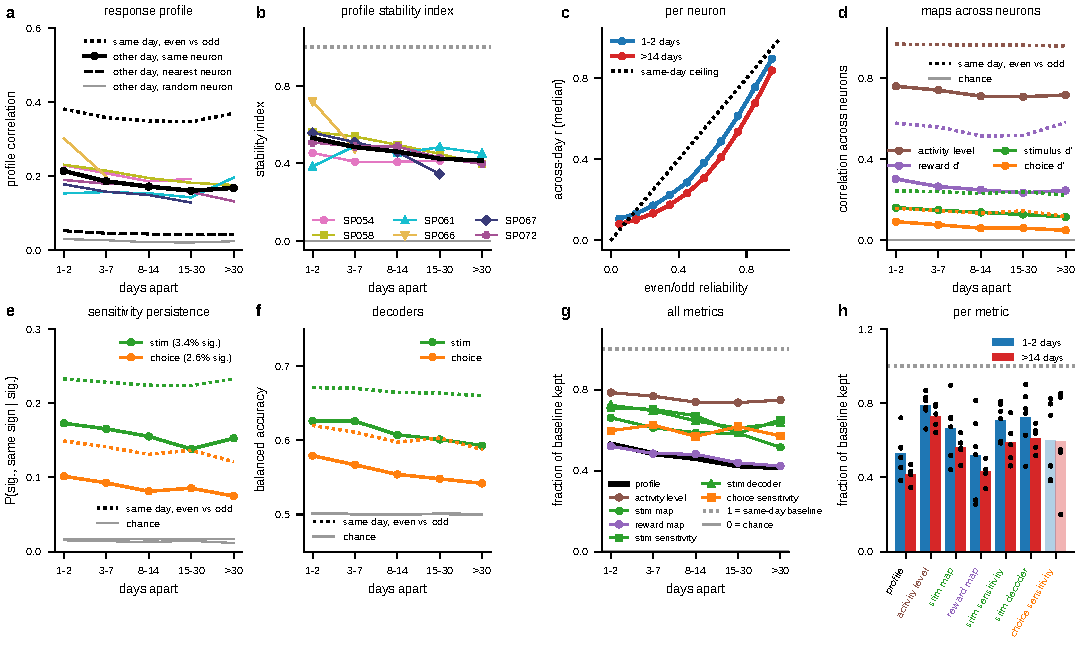
\includegraphics[width=\textwidth]{chronic_stability.pdf}
\caption{\textbf{Cross-day reliability of tracked neurons, each metric against its even/odd within-session baseline.}
6 mice, 83 sessions, 644 session pairs, QC-passing matches only. Line styles throughout: dotted, same-day baseline (even vs.\ odd trials of the same session); solid with markers, across days (even trials of day $a$ vs.\ odd trials of day $b$); thin grey, chance. Colours throughout: black, response profile; brown, activity level; green, stimulus; orange, choice; purple, reward; blue and red, 1--2 and $>$14 days apart (c, h). Thin coloured lines (a) and coloured markers (b): individual mice; thick black lines: mean over mice.
\textbf{a}~Median correlation of the 27-value response profile on the same day, with the same neuron on another day, with the spatially nearest tracked neuron (dashed) and with a random neuron of the same FOV (grey, chance).
\textbf{b}~Profile stability index $(r_x-r_0)/(r_w-r_0)$ per mouse, with medians over neurons of $r_w$ (within day, w: even vs.\ odd trials of the same session), $r_x$ (across days, x: even trials of day $a$ vs.\ odd trials of day $b$) and $r_0$ (chance, 0: as $r_x$ but with a random other neuron of the same FOV).
\textbf{c}~Per neuron: median across-day correlation $r_x$ against even/odd reliability $\sqrt{r_{w,a}\,r_{w,b}}$, the geometric mean of the neuron's within-day correlations on day $a$ and day $b$; dotted: identity, the across-day value expected from the same-day noise ceiling if the profile did not change.
\textbf{d}~Population maps: for each session half, one value per tracked neuron; the map is compared by Pearson correlation across the neurons shared by the two sessions. Activity level: $\log$ of the neuron's mean deconvolved activity over all trials and windows. $d'=(\mu_1-\mu_2)/\sqrt{(\sigma_1^2+\sigma_2^2)/2}$ of single-trial activity between two trial groups: stimulus, contra- vs.\ ipsilateral stimulus in the stimulus window (0--0.3\,s); choice, the two choices in the pre-movement window ($-0.3$--0\,s); reward, rewarded vs.\ unrewarded trials in the feedback window (0--0.3\,s).
\textbf{e}~Of the neurons significantly stimulus- or choice-selective on one half ($p<0.01$), the fraction significant with the same sign on the other half; grey: chance (half the fraction of significant neurons).
\textbf{f}~Ridge decoders of stimulus side and choice; grey: chance, from decoders trained on shuffled labels.
\textbf{g}~All metrics of a, b and d--f as the fraction of their baseline kept; colour, variable; marker, metric type (circles, maps; squares, sensitivity persistence; triangles, decoders). Dotted grey at 1: as reproducible as the same-day baseline; solid grey at 0: chance. The choice map and the choice decoder are not normalised: their within-session values are close to chance, so the per-pair ratio is ill-defined.
\textbf{h}~Fraction of baseline kept at 1--2 vs.\ $>$14 days apart, per metric (label colour as in g); bars: mean over mice; dots: mice (6 at 1--2 days, 5 at $>$14 days: SP066 spans 6 days); dotted: baseline. Choice sensitivity (faded) has a baseline close to chance and is unreliable.}
\label{fig:main}
\end{figure}
